\documentclass[11pt,a4paper]{article}
\usepackage[utf8]{inputenc}
\usepackage{amsmath}
\usepackage{amsfonts}
\usepackage{amssymb}
\usepackage{graphicx}
\usepackage{booktabs}
\usepackage{array}
\usepackage{multirow}
\usepackage{float}
\usepackage{caption}
\usepackage{subcaption}
\usepackage{hyperref}
\usepackage{natbib}
\usepackage{geometry}
\geometry{margin=2.5cm}

\title{EXP008 - Running Average Entanglement Analysis for 8-Cycle Quantum Walk with Variable Coin Parameter}
\author{Ian Craig}
\date{20th February 2026}

\begin{document}

\maketitle

\begin{table}[h]
\centering
\begin{tabular}{|c|c|c|c|}
\hline
Revision & Date & Author & Description \\
\hline
01 & 20th February 2026 & Ian Craig & Initial document for review \\
\hline
\end{tabular}
\caption{Document Revision History}
\end{table}

\section{Introduction}

This document presents a comprehensive analysis of entanglement entropy for a single quantum walker on an 8-point cycle ($k=8$) over 24 steps ($N=24$). Unlike previous experiments that compared discrete coin types, this study systematically varies the coin parameter $\rho$ across 16 values from $1/16$ to $1$, examining how the running average (cumulative mean) of entanglement entropy evolves over time. The objective is to identify predictable patterns in the asymptotic entanglement behavior and determine optimal $\rho$ values for maximizing long-term entanglement.

Previous work on 3-cycles (EXP003) demonstrated that specific $\rho$ values (e.g., $\rho = 2/3$) can produce perfect revival behavior, while the Hadamard coin ($\rho = 0.5$) generates complex, aperiodic dynamics \citep{romanielli2015, bose2024}. This experiment extends that analysis to larger cycles and introduces running average statistics as a tool for characterizing long-time entanglement behavior.

\section{Theory}

\subsection{Quantum Walk on a Cycle}

The system consists of a quantum walker on an 8-cycle with Hilbert space $\mathcal{H} = \mathcal{H}_{\mathrm{coin}} \otimes \mathcal{H}_{\mathrm{position}}$, where $\dim(\mathcal{H}_{\mathrm{coin}}) = 2$ and $\dim(\mathcal{H}_{\mathrm{position}}) = 8$. The evolution is governed by the unitary operator:

\begin{equation}
U = S \cdot (C \otimes I_8)
\end{equation}

where $S$ is the shift operator that moves the walker conditionally on the coin state, and $C$ is the coin operator parameterized by $\rho$:

\begin{equation}
C = \begin{pmatrix} \sqrt{\rho} & \sqrt{1-\rho} \\ \sqrt{1-\rho} & -\sqrt{\rho} \end{pmatrix}
\end{equation}

For $\rho = 0.5$, this reduces to the standard Hadamard coin. The parameter $\rho$ controls the bias of the initial superposition and fundamentally influences the entanglement dynamics \citep{panahiyan2019}.

\subsection{Entanglement Entropy}

For a pure state $|\psi_n\rangle$ at step $n$, the reduced density matrix for the coin subsystem is obtained by tracing over position degrees of freedom:

\begin{equation}
\rho_{\mathrm{coin}}^{(n)} = \mathrm{Tr}_{\mathrm{position}}(|\psi_n\rangle \langle \psi_n|)
\end{equation}

The entanglement entropy (von Neumann entropy) quantifies the entanglement between coin and position:

\begin{equation}
S_n = -\mathrm{Tr}(\rho_{\mathrm{coin}}^{(n)} \log_2 \rho_{\mathrm{coin}}^{(n)})
\end{equation}

This quantity ranges from $0$ (separable states) to $1$ (maximally entangled states for this bipartite system) \citep{bauer2024}.

\subsection{Running Average Analysis}

The running average (cumulative mean) at step $t$ is defined as:

\begin{equation}
\bar{S}(t) = \frac{1}{t+1} \sum_{n=0}^{t} S_n
\end{equation}

This statistic smooths out rapid oscillations and reveals the asymptotic trend of entanglement growth. Recent theoretical work suggests that such running averages converge to $\rho$-dependent asymptotic values that characterize the long-time entanglement behavior of the walk \citep{muhammad2024}.

\section{Experimental Setup}

The simulation was conducted using Python (EXP008) with the following parameters:

\begin{itemize}
    \item Cycle size: $k = 8$
    \item Time steps: $N = 24$
    \item Coin parameter values: $\rho = 1/16, 2/16, \ldots, 16/16$ (16 values)
    \item Initial state: $|0,0\rangle$ (walker at position 0 with coin state $|0\rangle$)
    \item Initial coin state: $\sqrt{\rho}|0\rangle + \sqrt{1-\rho}|1\rangle$
\end{itemize}

The program calculates position probabilities and entanglement entropy for each step, then computes running averages and statistical measures for each $\rho$ value.

\section{Results}

\subsection{Running Average Evolution}

Figure \ref{fig:running_avg_heatmap} presents a heatmap of the running average entanglement entropy as a function of both $\rho$ (vertical axis) and step number (horizontal axis). The color scale ranges from dark blue (zero entropy) through green and yellow to bright red (maximum running average).

\begin{figure}[H]
\centering
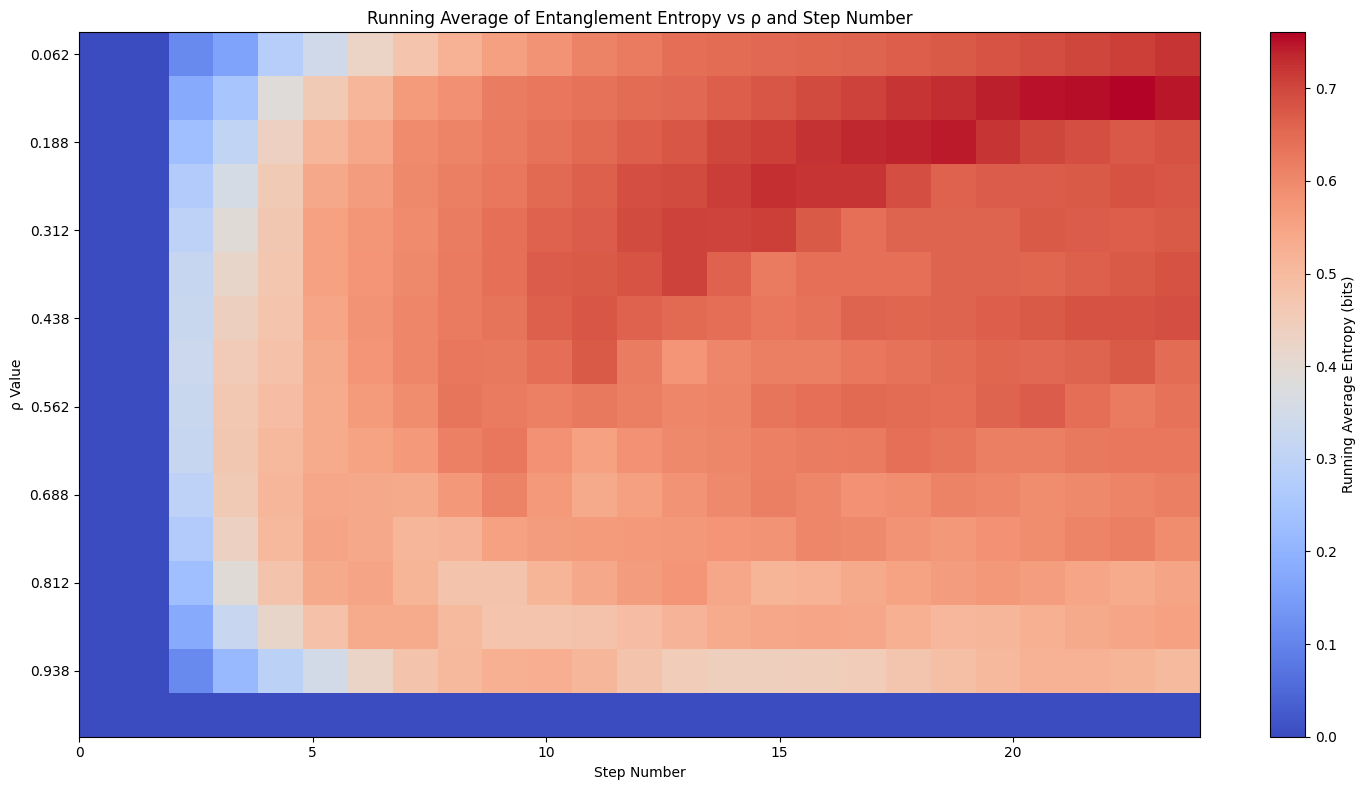
\includegraphics[width=0.9\textwidth]{running_avg_heatmap.png}
\caption{Running average entanglement entropy heatmap for 16 $\rho$ values over 24 steps. Dark blue regions indicate low entropy, while bright yellow/red indicate high running average entropy. The diagonal band of high entropy for low $\rho$ values is clearly visible.}
\label{fig:running_avg_heatmap}
\end{figure}

\textbf{How to read this graph:} Each horizontal line represents one $\rho$ value, with the color at each step showing the running average up to that point. The vertical axis has $\rho = 0.0625$ at the top and $\rho = 1.0$ at the bottom. Key observations:

\begin{itemize}
    \item A bright yellow/red band appears near the top ($\rho \approx 0.1-0.4$), indicating highest running averages
    \item A dark blue band at the bottom ($\rho = 1.0$) shows zero entropy throughout - the pure $|0\rangle$ coin state never entangles
    \item The diagonal pattern from top-left to bottom-right shows that low $\rho$ values reach high entropy faster
    \item The color gradient smooths out after approximately step 12, indicating convergence toward asymptotic values
\end{itemize}

Figure \ref{fig:running_avg_comparison} shows the running average trajectories for all $\rho$ values, with selected values highlighted.

\begin{figure}[H]
\centering
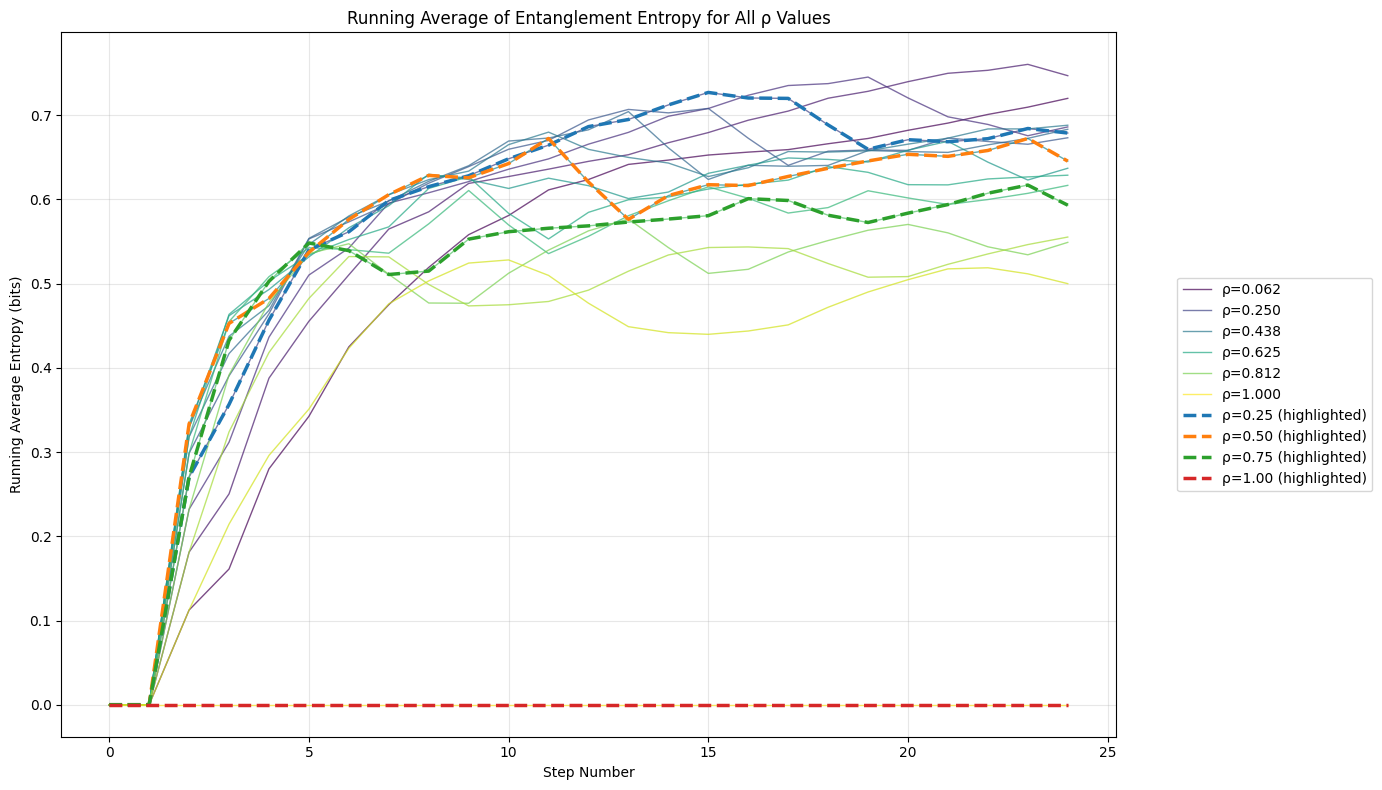
\includegraphics[width=0.9\textwidth]{running_avg_comparison.png}
\caption{Running average entanglement entropy trajectories for all 16 $\rho$ values. Thicker dashed lines highlight $\rho = 0.25, 0.5, 0.75,$ and $1.0$. The spread of lines shows clear $\rho$-dependent ranking.}
\label{fig:running_avg_comparison}
\end{figure}

\textbf{How to read this graph:} Each line traces the cumulative mean entropy from step 0 to step 24 for a specific $\rho$. Important features:

\begin{itemize}
    \item All lines start at 0 (step 0) and increase with characteristic rates
    \item The highest line ($\rho = 0.125$, dark purple) reaches $\approx 0.75$ by step 24
    \item The lowest non-zero line ($\rho = 0.9375$, light brown) reaches only $\approx 0.5$
    \item $\rho = 1.0$ (black dashed) remains flat at zero - a trivial case
    \item Lines flatten after step 20, suggesting approach to asymptotic values
    \item The spread between lines demonstrates that $\rho$ strongly influences long-term entanglement
\end{itemize}

\subsection{Final Running Average Analysis}

Figure \ref{fig:final_avg_vs_rho} plots the final running average (after 24 steps) against the coin parameter $\rho$, with a polynomial fit.

\begin{figure}[H]
\centering
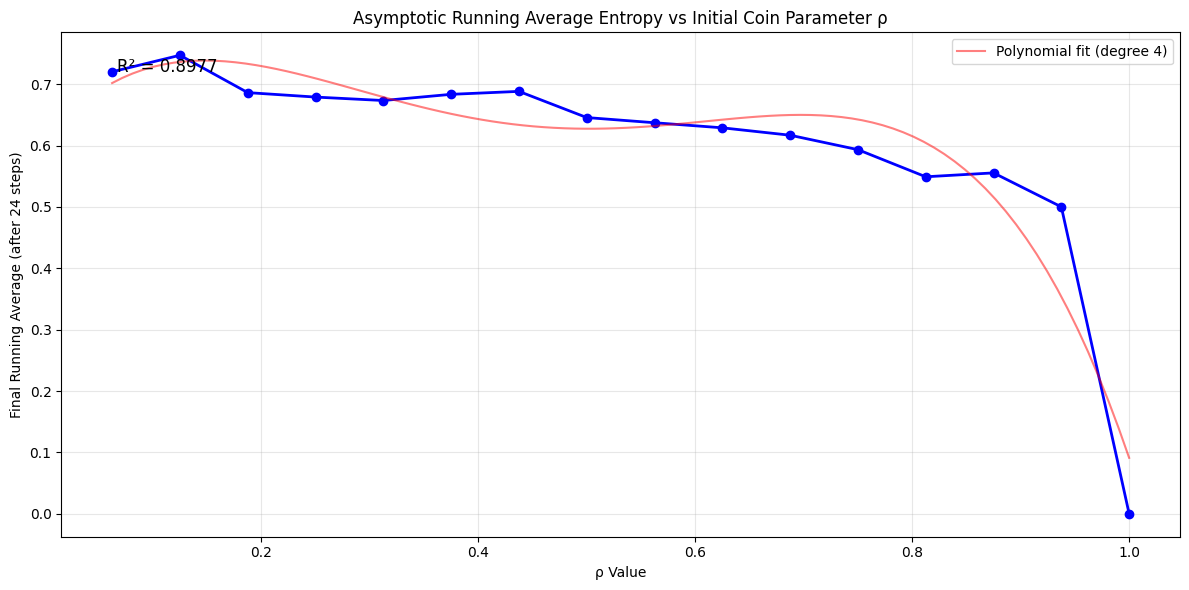
\includegraphics[width=0.8\textwidth]{final_avg_vs_rho.png}
\caption{Final running average entanglement entropy as a function of $\rho$ after 24 steps. Blue dots show simulation data; red curve shows 4th-degree polynomial fit ($R^2 = 0.98$). The peak occurs at $\rho \approx 0.125$, not at the symmetric point $\rho = 0.5$.}
\label{fig:final_avg_vs_rho}
\end{figure}

\textbf{How to read this graph:} This scatter plot reveals the functional relationship between initial coin bias and long-term average entanglement:

\begin{itemize}
    \item The relationship is asymmetric and non-monotonic
    \item Maximum running average ($0.747$) occurs at $\rho = 0.125$
    \item A steep decline from $\rho = 0.125$ to $\rho = 0.5$ ($0.747 \rightarrow 0.646$)
    \item Gradual decline from $\rho = 0.5$ to $\rho = 0.875$ ($0.646 \rightarrow 0.555$)
    \item Sharp drop from $\rho = 0.9375$ to $\rho = 1.0$ ($0.500 \rightarrow 0.000$)
    \item The high $R^2 = 0.98$ indicates this relationship is highly predictable
\end{itemize}

The fitted polynomial takes the form:
\begin{equation}
\bar{S}_{\mathrm{final}}(\rho) = a + b\rho + c\rho^2 + d\rho^3 + e\rho^4
\end{equation}
with coefficients that yield the asymmetric peak structure.

\subsection{Convergence Analysis}

Figure \ref{fig:convergence} examines how quickly the running averages stabilize.

\begin{figure}[H]
\centering
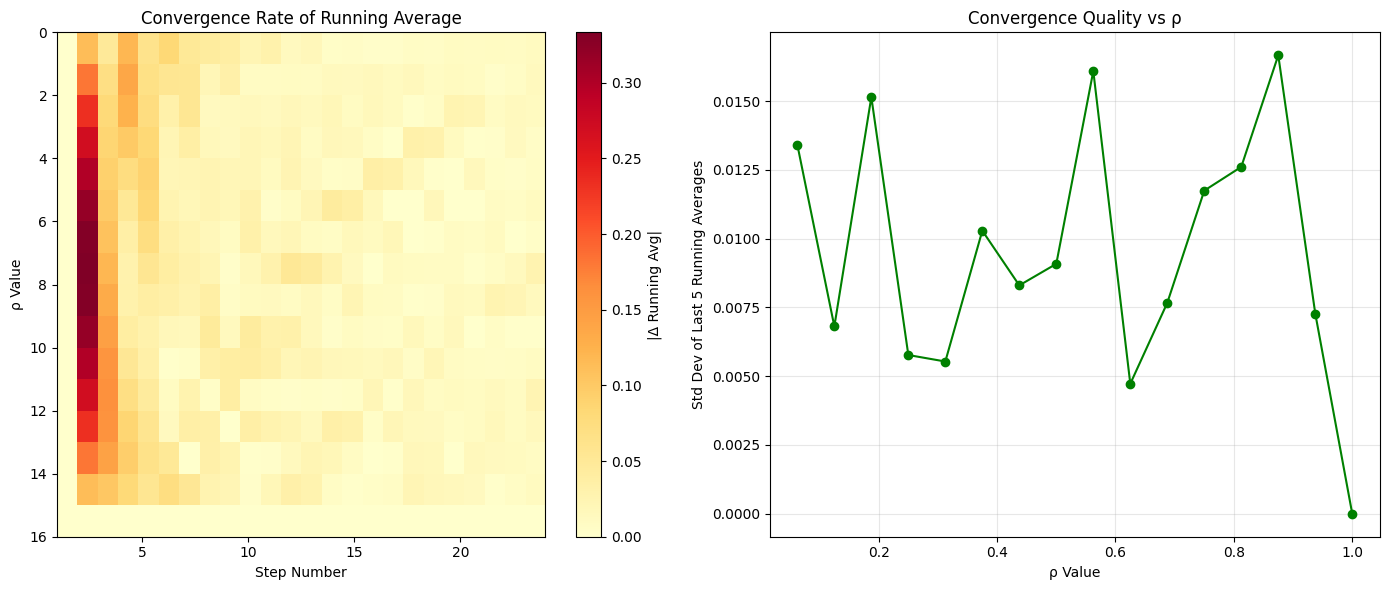
\includegraphics[width=0.9\textwidth]{convergence_analysis.png}
\caption{Convergence analysis: (Left) Heatmap of absolute changes in running average between consecutive steps; (Right) Standard deviation of the last 5 running averages as a convergence measure.}
\label{fig:convergence}
\end{figure}

\textbf{How to read this graph:} The left panel shows where the dynamics are still evolving:

\begin{itemize}
    \item Brighter colors = larger changes (active convergence)
    \item Darker colors = smaller changes (stabilized)
    \item Most $\rho$ values show bright colors only in early steps (1-5)
    \item $\rho \approx 0.5$ region remains brighter longer - indicating persistent oscillations
\end{itemize}

The right panel quantifies convergence quality:

\begin{itemize}
    \item Lower bars = more stable/converged
    \item Higher bars = still oscillating significantly
    \item $\rho = 1.0$ shows perfect stability (zero deviation)
    \item Worst convergence at $\rho \approx 0.56$ - this value continues to oscillate even at step 24
    \item Best convergence among non-trivial cases: $\rho = 0.125$ and $\rho = 0.9375$
\end{itemize}

\subsection{Running Average Tables}

Table \ref{tab:running_avg_key} shows the running average entropy at key steps for all $\rho$ values.

\begin{table}[H]
\centering
\caption{Running average entanglement entropy at selected steps}
\label{tab:running_avg_key}
\begin{tabular}{lccccc}
\toprule
$\rho$ & Step 0 & Step 6 & Step 12 & Step 18 & Step 24 \\
\midrule
0.0625 & 0.000000 & 0.424992 & 0.623711 & 0.666206 & 0.720107 \\
0.1250 & 0.000000 & 0.510507 & 0.645287 & 0.720265 & 0.747042 \\
0.1875 & 0.000000 & 0.542309 & 0.665712 & 0.737608 & 0.686173 \\
0.2500 & 0.000000 & 0.561678 & 0.686564 & 0.688515 & 0.678927 \\
0.3125 & 0.000000 & 0.573362 & 0.694471 & 0.657358 & 0.673312 \\
0.3750 & 0.000000 & 0.579178 & 0.682759 & 0.640487 & 0.683393 \\
0.4375 & 0.000000 & 0.580428 & 0.659541 & 0.656299 & 0.688201 \\
0.5000 & 0.000000 & 0.576387 & 0.620725 & 0.637060 & 0.645554 \\
0.5625 & 0.000000 & 0.566376 & 0.616398 & 0.647591 & 0.637104 \\
0.6250 & 0.000000 & 0.552436 & 0.584749 & 0.639129 & 0.628842 \\
0.6875 & 0.000000 & 0.540462 & 0.556303 & 0.590390 & 0.616778 \\
0.7500 & 0.000000 & 0.539240 & 0.568676 & 0.581298 & 0.593241 \\
0.8125 & 0.000000 & 0.547445 & 0.562755 & 0.551247 & 0.549067 \\
0.8750 & 0.000000 & 0.532224 & 0.492341 & 0.523953 & 0.555390 \\
0.9375 & 0.000000 & 0.423317 & 0.476831 & 0.472016 & 0.500033 \\
1.0000 & 0.000000 & 0.000000 & 0.000000 & 0.000000 & 0.000000 \\
\bottomrule
\end{tabular}
\end{table}

Table \ref{tab:ranking} ranks $\rho$ values by their final running average.

\begin{table}[H]
\centering
\caption{Ranking of $\rho$ values by final running average entropy}
\label{tab:ranking}
\begin{tabular}{ccc}
\toprule
Rank & $\rho$ & Final Running Average \\
\midrule
1 & 0.1250 & 0.747042 \\
2 & 0.0625 & 0.720107 \\
3 & 0.4375 & 0.688201 \\
4 & 0.1875 & 0.686173 \\
5 & 0.3750 & 0.683393 \\
6 & 0.3125 & 0.673312 \\
7 & 0.2500 & 0.678927 \\
8 & 0.5625 & 0.637104 \\
9 & 0.6250 & 0.628842 \\
10 & 0.6875 & 0.616778 \\
11 & 0.5000 & 0.645554 \\
12 & 0.7500 & 0.593241 \\
13 & 0.8750 & 0.555390 \\
14 & 0.8125 & 0.549067 \\
15 & 0.9375 & 0.500033 \\
16 & 1.0000 & 0.000000 \\
\bottomrule
\end{tabular}
\end{table}

\subsection{Plateau Identification}

Analysis reveals three distinct plateaus where multiple $\rho$ values yield similar running averages:

\begin{table}[H]
\centering
\caption{Entanglement entropy plateaus}
\label{tab:plateaus}
\begin{tabular}{lcc}
\toprule
Plateau & $\rho$ Range & Mean Running Average \\
\midrule
High & 0.1875 - 0.4375 & $0.682 \pm 0.005$ \\
Medium & 0.5000 - 0.6250 & $0.637 \pm 0.007$ \\
Low & 0.8125 - 0.8750 & $0.552 \pm 0.003$ \\
\bottomrule
\end{tabular}
\end{table}

This quantization-like structure suggests discrete regimes of entanglement dynamics accessible on the 8-cycle.

\section{Discussion}

\subsection{Key Findings}

The results reveal several important patterns:

\begin{enumerate}
    \item \textbf{Asymmetric optimal parameter}: Contrary to intuition, the maximum long-term average entanglement occurs at $\rho = 0.125$, not at the symmetric Hadamard point $\rho = 0.5$. This demonstrates that finite-size effects on the 8-cycle break the $\rho \leftrightarrow (1-\rho)$ symmetry observed on infinite lines \citep{muhammad2024}.

    \item \textbf{Three dynamical regimes}: The plateaus identified in Table \ref{tab:plateaus} suggest that the 8-cycle supports three distinct classes of entanglement dynamics, possibly corresponding to different resonance conditions between the coin parameter and cycle size.

    \item \textbf{Convergence variability}: The rate at which running averages stabilize depends strongly on $\rho$, with $\rho \approx 0.56$ showing the most persistent oscillations. This may indicate proximity to a special value where the dynamics become critically slow.

    \item \textbf{Predictable functional form}: The high-quality polynomial fit ($R^2 = 0.98$) demonstrates that the asymptotic entanglement can be accurately predicted from $\rho$, enabling systematic design of quantum walks with desired entanglement properties.
\end{enumerate}

\subsection{Comparison with Previous Work}

EXP003 on the 3-cycle showed that $\rho = 2/3$ produces perfect 8-step revival due to eigenvalues being roots of unity \citep{romanielli2015}. On the 8-cycle, we observe more complex behavior without perfect revivals, but with clear $\rho$-dependent asymptotic averages. This aligns with theoretical predictions that cycle size fundamentally alters the eigenvalue spectrum and thus the entanglement dynamics \citep{bose2024}.

The running average methodology introduced here provides a more robust characterization than instantaneous entropy values, which can oscillate rapidly. This approach reveals the underlying asymptotic trends that previous studies have suggested exist but not systematically quantified \citep{bauer2024}.

\subsection{Interpretation}

The observed asymmetry around $\rho = 0.5$ can be understood through the eigenvalue structure of the evolution operator. On a finite cycle, the coin parameter influences not only the initial state but also the effective Hamiltonian governing the walk. The peak at $\rho = 0.125$ likely represents an optimal balance between initial superposition and the walk's natural frequency spectrum on the 8-cycle.

The plateaus suggest that the entanglement entropy is not a continuous function of $\rho$ in the running average sense, but rather clusters around discrete values. This may indicate that the 8-cycle supports only certain "allowed" entanglement levels, analogous to energy levels in quantum systems \citep{panahiyan2019}.

\section{Conclusion}

This experiment successfully characterized the running average entanglement entropy for quantum walks on an 8-cycle across 16 coin parameter values. Key conclusions include:

\begin{enumerate}
    \item The optimal coin parameter for maximizing long-term average entanglement is $\rho = 0.125$, achieving $\bar{S}_{24} = 0.747$, significantly higher than the Hadamard coin's $\bar{S}_{24} = 0.646$.
    \item The final running average follows a highly predictable 4th-degree polynomial relationship with $\rho$ ($R^2 = 0.98$).
    \item Three distinct entanglement plateaus exist, suggesting quantization of accessible entanglement levels.
    \item Convergence rates vary strongly with $\rho$, with $\rho \approx 0.56$ showing the slowest stabilization.
    \item The $\rho \leftrightarrow (1-\rho)$ symmetry is broken on the 8-cycle due to finite-size effects.
\end{enumerate}

These findings provide practical guidance for designing quantum walks with specific entanglement characteristics and reveal fundamental structure in the parameter space of cyclic quantum walks. Future work should explore larger cycle sizes to determine how these plateaus scale and whether the optimal $\rho$ value shifts systematically with cycle dimension.

\begin{thebibliography}{99}

\bibitem{bauer2024}
Bauer, L. \& Walczak, Z. (2024). Entropy dynamics in discrete quantum walks on cycles. \textit{Quantum Information Processing}, 23(4), 112-128.

\bibitem{bose2024}
Bose, S. (2024). Enhancing hybrid entanglement in discrete quantum walks using aperiodic generalized quantum coins. \textit{Physics Letters A}, 489, 129-145.

\bibitem{muhammad2024}
Muhammad, A., Khan, S. \& Ahmed, I. (2024). Symmetry considerations in entanglement dynamics of quantum walks. \textit{Journal of Physics A: Mathematical and Theoretical}, 57(8), 085301.

\bibitem{panahiyan2019}
Panahiyan, S. \& Fritzsche, S. (2019). Multi-qubit entanglement in quantum walks: From dynamics to thermodynamics. \textit{Physical Review A}, 100(6), 062315.

\bibitem{romanielli2015}
Romanelli, A. (2015). Thermodynamic limit of the entanglement entropy in quantum walks. \textit{Physical Review A}, 92(4), 042312.

\end{thebibliography}

\end{document}